\documentclass{article}
\usepackage[utf8]{inputenc}

\title{Hilos}
\author{Chrsitian Gallego Chaverra}
\date{July 2020}

\usepackage{natbib}
\usepackage{graphicx}

\begin{document}

\maketitle

\section{¿Que son los Hilos?}
Un hilo es una línea de ejecución de un proceso. Todo proceso parte inicialmente con un único hilo principal, aunque el sistema operativo ofrece llamadas al sistema que permiten al programador crear y destruir hilos. Por tanto, un proceso está compuesto por uno o más hilos.
Podemos definir un hilo de procesamiento como el flujo de control de datos de un programa. Es un medio que permite administrar las tareas de un procesador y de sus diferentes núcleos de una forma más eficiente. Gracias a los hilos, las unidades mínimas de asignación, que son las tareas o procesos de un programa, pueden dividirse en trozos para así optimizar los tiempos de espera de cada instrucción en la cola del proceso. Estos trozos se llaman subprocesos o threads.
Dicho de otra forma, cada hilo de procesamiento contiene un trozo de la tarea a realizar, algo más simple de realizar que si introducimos la tarea completa en el núcleo físico. De esta forma la CPU es capaz de procesar varias tareas al mismo tiempo y de forma simultánea, de hecho, podrá hacer tantas tareas como hilos tenga, y normalmente son una o dos por cada núcleo. En los procesadores que tienen por ejemplo 6 núcleos y 12 hilos serán capaces de dividir los procesos en 12 tareas distintas en lugar de solamente 6\cite{intro}.

\begin{figure}[h!]
\centering
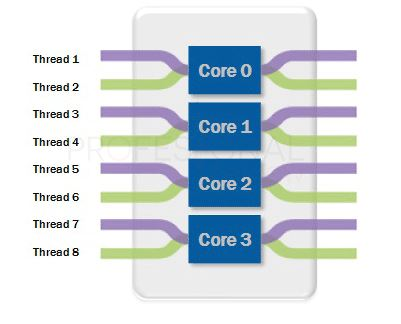
\includegraphics[scale=0.9]{hilos.JPG}
\caption{Hilos de un procesador.\cite{intro}}
\label{fig:hilos}
\end{figure}

Los hilos se distinguen de los tradicionales procesos en que los procesos son –generalmente– independientes, llevan bastante información de estados, e interactúan solo a través de mecanismos de comunicación dados por el sistema. Por otra parte, muchos hilos generalmente comparten otros recursos de forma directa. En muchos de los sistemas operativos que dan facilidades a los hilos, es más rápido cambiar de un hilo a otro dentro del mismo proceso, que cambiar de un proceso a otro. Este fenómeno se debe a que los hilos comparten datos y espacios de direcciones, mientras que los procesos, al ser independientes, no lo hacen.

\section{Tipos de hilos}

\bibliographystyle{plain}
\bibliography{references}
\end{document}
